\documentclass[10pt,a4paper]{article}
\usepackage[utf8]{inputenc}
\usepackage[brazilian]{babel}
\usepackage[left=2cm, right=2cm, top=2cm, bottom=2cm]{geometry}
\usepackage[problem-list]{zeus}
\usepackage{parskip}
\usepackage{transparent}
\usepackage{lmodern}
\usepackage{multicol}
\usepackage[euler-digits, euler-hat-accent]{eulervm}

\setlength{\columnsep}{3em}

\title{Tutoria, 18:00}
\author{Guilherme Zeus Dantas e Moura}
\mail{zeusdanmou@gmail.com}
\titlel{\rlap{Matematicamente Internacionais}\smash{\raisebox{-2.4cm}{\transparent{.3}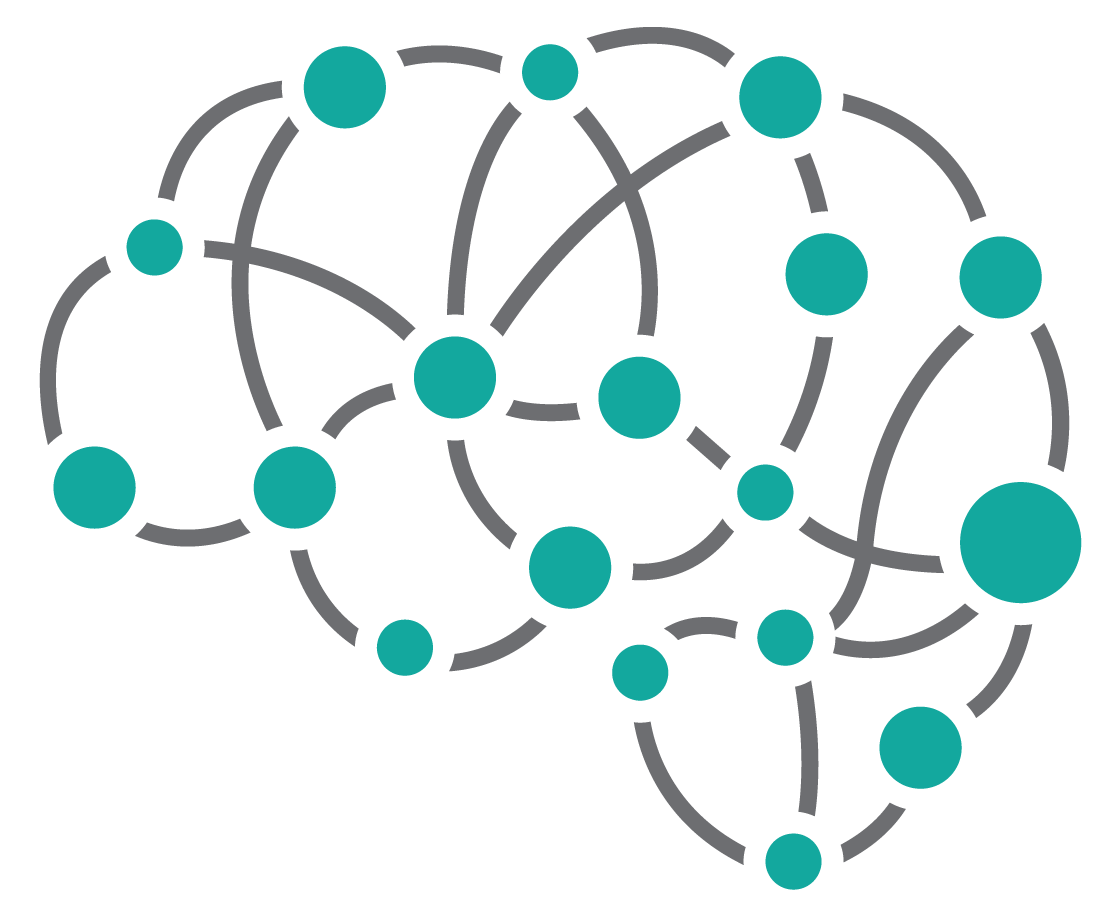
\includegraphics[width = 3cm]{mm_2}}}}
\titler{29 de Maio de 2021}

\pagestyle{empty}

\begin{document}	
 	\zeustitle

	\problem*{math/imosl/2015/G3}
	\begin{sol}
		Defina $\Gamma$ como o circuncírculo de $ABC$.
		Defina $X$ como a projeção de $D$ sobre $AB$. Note que $AH = HX$.
		Defina $Z$ como a intersecção de $AD$ e $\omega$. Como $90^\circ = \angle DZB = \angle AZB$,  $Z \in \Gamma$.

		Defina $Q'$ como a segunda intersecção de $CZ$ com $\omega$. Como $Q' \in \omega$, vale que $\angle BQ'D = 90^\circ$. Note que $\angle ABC = \angle AZC = \angle DZQ' = \angle DBQ'$. Portanto, por ângulo-ângulo, $\triangle BCA \sim \triangle BQ'D$.

		Seja $\phi$ a rotohomotetia que leva $\triangle BCA$ em $\triangle BQ'D$. A transformação $\phi$ possui centro $B$ e $\angle ABD$. 
		Tome $T$ como a intersecção da tangente a $\Gamma$ por $C$ com a reta $AB$. Vamos mostrar que $\phi$ leva $T$ em $P$.

		A condição dos ângulos é verdade, pois $\angle TBP = \angle ABD$, que é o ângulo da rotohomotetia.
		A condição das razões também é verdade, pois temos que  \[
			\frac{TA}{TB} = \frac{TA}{TC}\cdot\frac{TC}{TB} = \left(\frac{AC}{BC}\right)^2 = \frac{AC\cdot\cos\angle A}{BC\cdot\cos\angle B} = \frac{AH}{HB} = \frac{HX}{HB} = \frac{PD}{PB}.
		\]

		Portanto, de fato, $\phi$ leva $T$ em $P$ e, consequentemente, leva a tangente $TC$ ao circulo $\Gamma$ na reta tangente $PQ'$ a $\omega$. Logo, $Q' \equiv Q$.  
		Finalmente, as retas $AD$ e $CQ$ se intersectam em $Z$, que está sobre $\omega$.
	\end{sol}
	\problem*{math/imosl/2015/A2}

\end{document}
